\chapter{Additional Results}\label{sec:res_add}

This chapter showcases supplementary results to \sref{sec:exps}.

\section{SIS on a $G(n, p)$ network}\label{sec:res_gnp}

Results for SIS dynamics run on a $G(n, p)$ network.


\begin{figure}[H]
  \centering
  \makebox[\textwidth][c]{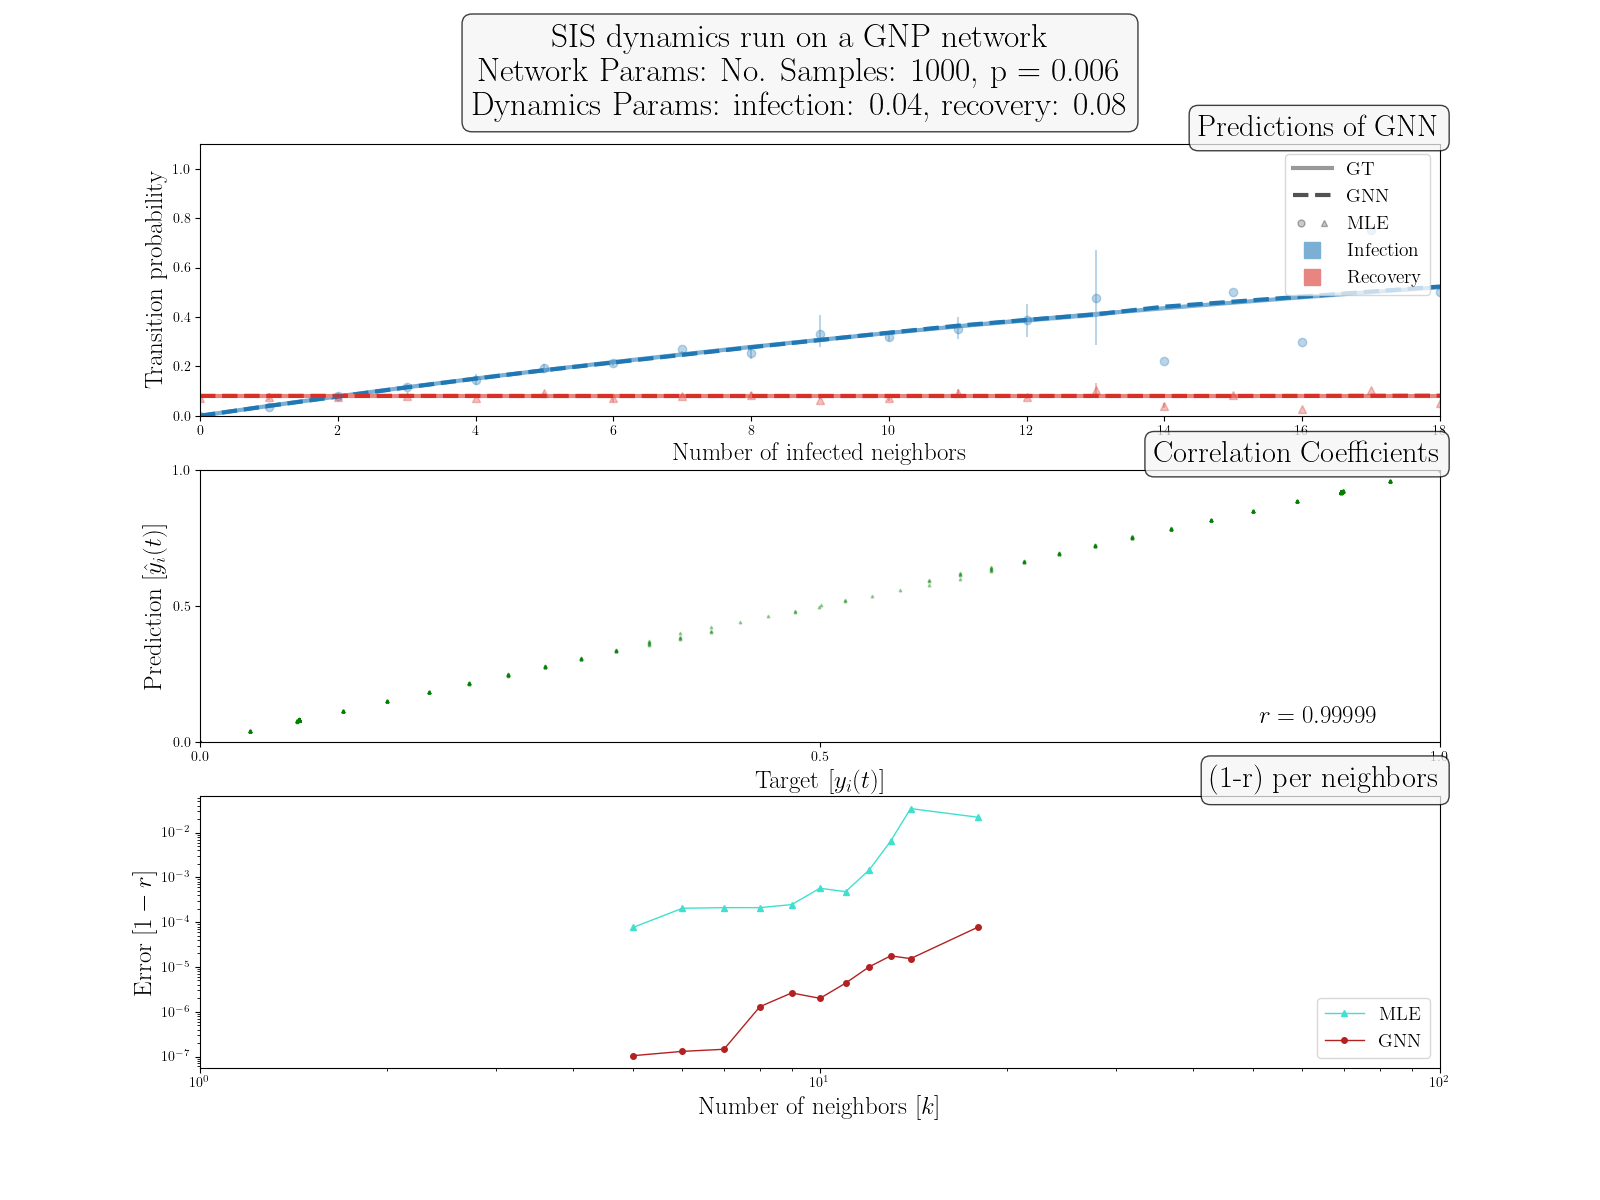
\includegraphics[width=1.4\textwidth]{Figures/chap_exp/gnp_sis_default.png}}
  \caption[Results for $G(n,p)$ network running SIS dynamics]{
    On the \textbf{top }figure, the transition probabilities for the simple
    contagion dynamics (SIS) dynamics model are shown. \textit{GT} stands
    for ground truth; the transition probabilities used when generating
    the dataset. Circles and triangles represent the MLE computed for said
    probabilities, with circles for the $S \rightarrow I$ transition and
    triangles for $I \rightarrow S$ with error bars present. The colored
    area around the lines is the standard deviation for a given number of
    infected neighbors. On the \textbf{middle} figure, a comparison of
    the predicted and targets ($y_i(t), \hat(y)_i(t)$) appears, with the Pearson
    coefficient $r$ for the whole set of pairs. Each point in this figure represents
    a different pair. On the \textbf{bottom} figure, the errors (1 - $r$) as a function
    of the number of neighbors are presented, both for the GNN and the MLE. These errors
    are computed from the subsets of the prediction and targets pairs where all
    nodes have degree $k$.
  }
  \label{fig:gnp_sis}
\end{figure}